\documentclass{sig-alternate}
\usepackage{textcomp}
\usepackage{graphics}

\begin{document}

\title{Redes Neuronales - Perceptr\'on Simple}
\subtitle{Sistemas de Inteligencia Artifical - ITBA}

\numberofauthors{3}

\author{
	\alignauthor{Carlos Sessa}\\
	\alignauthor{Lucas Pizzagalli}\\
	\alignauthor{Nicol\'as Purita}\\	
}

\date{12 de Abril de 2012}

\maketitle

\begin{abstract}
	Se implement\'o una red neuronal con aprendizaje supervisado que resuelve los operadores \textit{OR}  y \textit{AND} l\'ogicos, donde posee \textit{N} (con $2\leq N \leq 5$) entradas con \textit{1} salida.\\
\end{abstract}

\section*{Desarrollo}

La implementaci\'on del perceptr\'on simple se separa en tres funciones principales:
	\begin{equation}
		\label{learn}
			[ w_{out} ] = learn( g, g', w, input, expected, \eta )
		\end{equation}
		\begin{equation}
		\label{calculate}
			[ output ] = calculate( g, w, input )
		\end{equation}
		\begin{equation}
		\label{test}
			[ error ] = calculateError( g, w, input, expected)
		\end{equation}
Donde \textit{g} es la funci\'on de activaci\'on, \textit{g'} su derivada, \textit{input} son los patrones utilizados para el entrenamiento del perceptr\'on, \textit{expected} es la salida esperada, $\eta$ es la constante de proporcionalidad de aprendizaje y \textit{w} el vector de pesos. \\
La funci\'on \ref{learn} se utiliza para entrenar el perceptr\'on simple con un determinado patr\'on y retorna el vector de pesos correspondiente al mismo. \\
La funci\'on \ref{test} calcula el error en una \'epoca en sentido de cuadrados m\'inimos. Esta funci\'on es la encargada de determinar si es necesario continuar con el entrenamiento de la red, la decisi\'on es tomada en base a un cota de error determinada. \\
La funci\'on \ref{calculate} es la encargada de calcular la salida de la red una vez finalizado el entrenamiento. \\
Las pruebas se realizan variando la funci\'on de activaci\'on, el $\eta$ y manteniendo una cota de error de $0.01$. Cabe destacar que el orden en que se muestran los patrones a la red es aleatorio.

\section*{Problemas encontrados}
En un principio tuvimos inconvenientes por la utilizaci\'on de los n\'umeros binarios para la representaci\'on de la entrada y salida esperada. Esto se not\'o en la correcci\'on de los pesos ya que en ciertos casos la variaci\'on era 0. La causa de este problema es que la entrada es 0 generando que toda la variaci\'on de un peso d\'e 0. Para solucionarlo se realiza una transformaci\'on de entrada, para que todos los valores en 0 sean mapeados a -1. \\
Otro problema encontrado se deriva del anterior, ya que la funci\'on de activaci\'on exponencial al tener en la entrada un -1 no provocaba ninguna variaci\'on en el error, es decir, se saturaba la red neuronal. Para solucionarlo evitamos la transformaci\'on de la entrada. \\
Por otro lado, como luego se observar\'a en los resultados, la red se saturaba en valores incorrectos al utlizar algunas funciones de activaci\'on, por lo que nunca se alcanzaba un estado satisfactorio. Es por esto, que se debi\'o fijar una pol\'itica de corte. La misma se basa en que si el error es muy grande (en nuestro caso se decidi\'o $error > 10\epsilon$), pero el error var\'ia muy poco entre las distintas \'epocas, entonces significa que la red se encuentra saturada en una configuraci\'on err\'onea. Teniendo todo esto en cuenta, se decidio por la siguiente condici\'on de corte:
	\begin{equation}
		error\_var <  0.0000001 \&\& -0.09 < error - \epsilon > 0.1
	\end{equation} 
donde $error\_var$ es la diferencia cuadrada entre el promedio de las \'ultimas 200 \'epocas y el error de la \'epoca actual.
\section*{Resultados obtenidos}
Como se puede observar, no fue posible aprender ninguno de los operadores con la funci\'on lineal, sin embargo, el objetivo fue alcanzado por el resto de las funciones. Por otro lado, al utilizar la funci\'on de activaci\'on escal\'on, se llega a la soluci\'on rapidamente, mientras que utlizando la sigmoidea, el resultado es alcanzado m\'as lentamente. Otro dato apreciable, es que por lo general, al utilizar un $\eta$ mayor, se obtiene un aprendizaje m\'as r\'apido.
\section*{Conclusiones}
A simple vista se puede observar, que los comportamientos de todas las funciones de activaci\'on son muy similares tanto en el aprendizaje de la funci\'on \textit{OR} como la del \textit{AND}, ya que son problemas muy similares y linealmente separables. Tambi\'en se puede observar, que a mayor cantidad de entradas, le es mas dif\'icil a la red aprender lo deseado, debido a que hay mas variables a las que atender. Como se puede observar en los gr\'aficos de las que se ulitiz\'o la funci\'on lineal, no se logra el aprendizaje con el error querido, esto se debe a que dicha funci\'on no posee transformaciones apreciables para poder corregir los pesos de forma adecuada. Por \'ultimo, es importante destacar, que los $\eta$s m\'as grandes aceleran el aprendizaje sin mayores consecuencias debido a que se trata de problemas muy sencillos, en caso contrario, podr\'ian causar estancamiento.

% --------------------- Con N = 5 --------------------------------
\begin{figure}[!ht]
	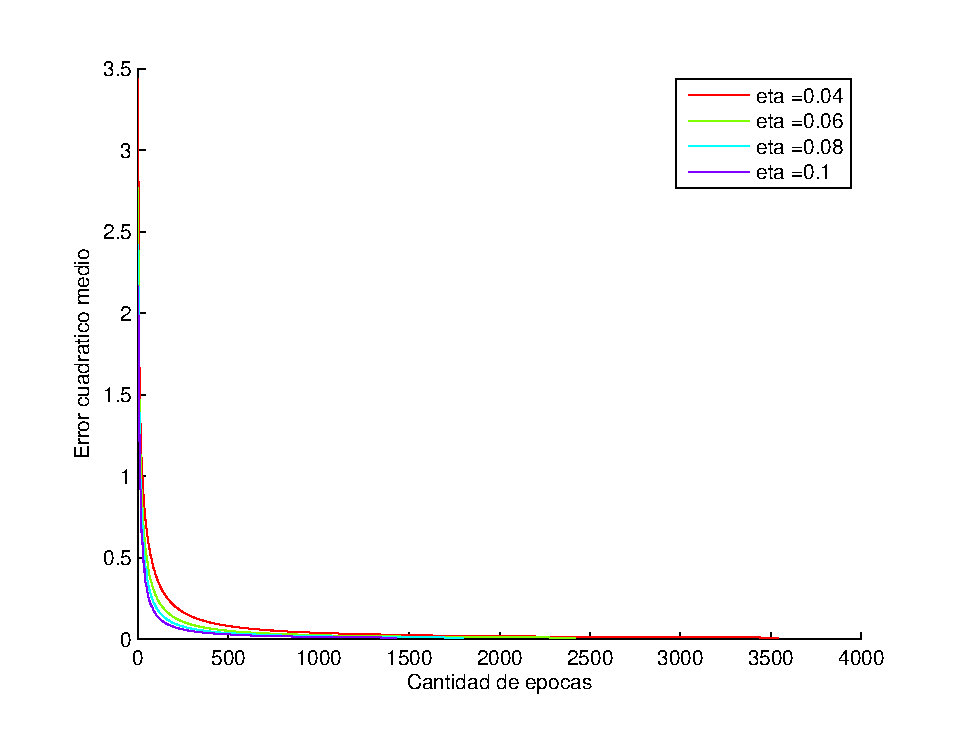
\includegraphics[scale=0.5]{images/PuriAnd/AND_N5_err001_tanh.eps}
  \caption{Funci\'on AND, N = 5 y funci\'on de activaci\'on $g(h) = tanh(\beta h)$}
  \label{fig:tanh}
\end{figure}

\begin{figure}[!ht]
	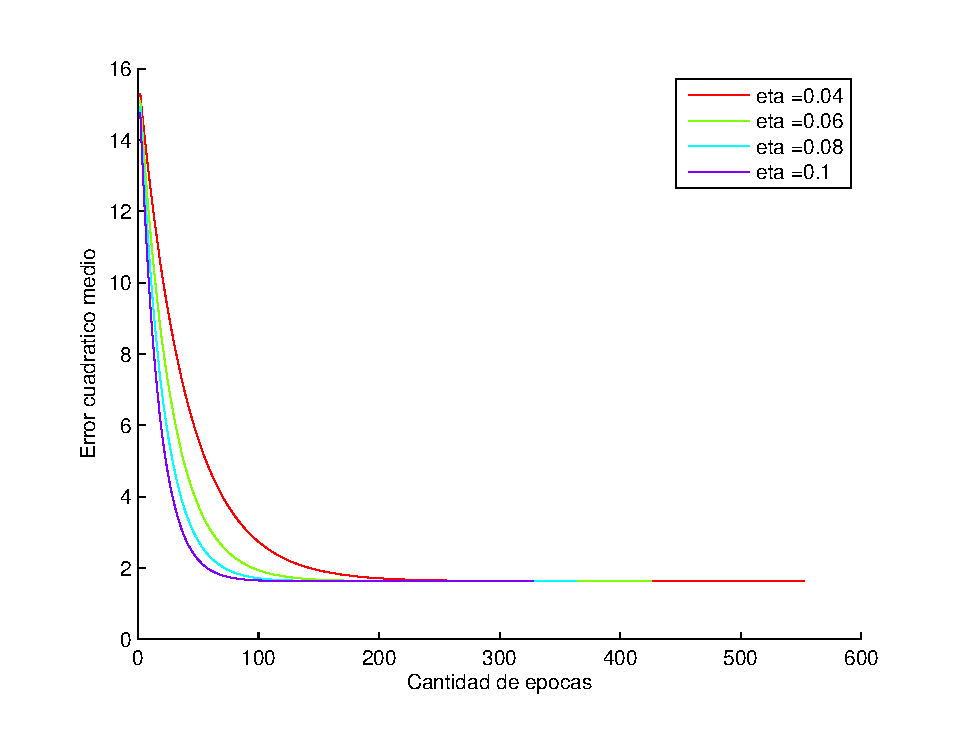
\includegraphics[scale=0.5]{images/PuriAnd/AND_N5_err001_lineal__error.eps}
  \caption{Funci\'on AND, N = 5 y funci\'on de activaci\'on $g(h) = h$}
  \label{fig:lineal}
\end{figure}

\begin{figure}[!ht]
	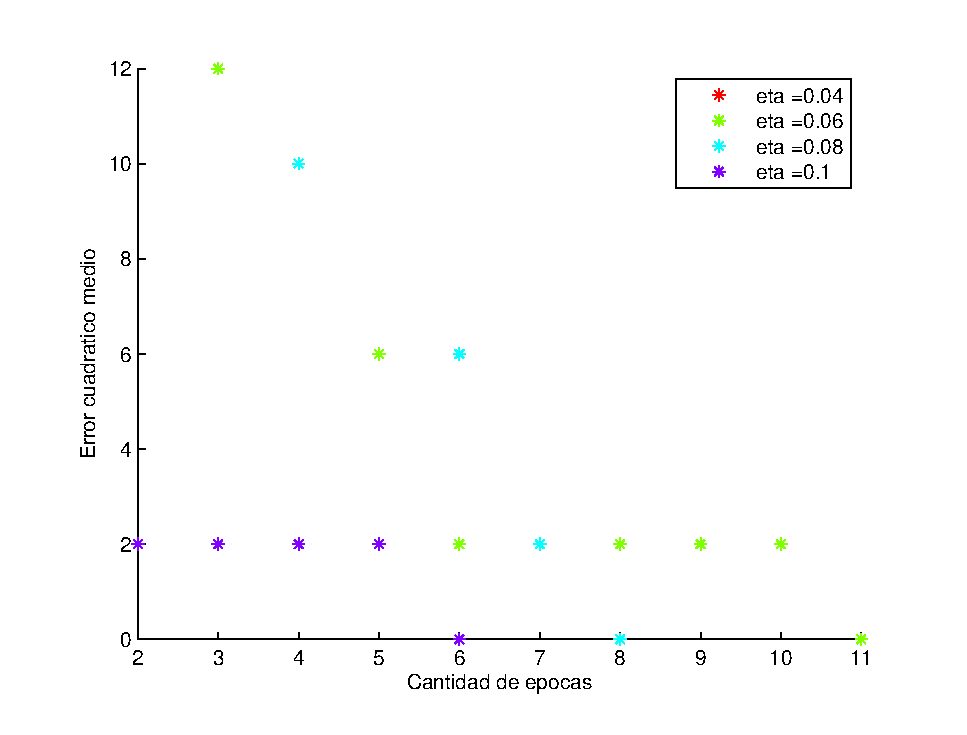
\includegraphics[scale=0.5]{images/PuriAnd/AND_N5_err001_step.eps}
  \caption{Funci\'on AND, N = 5 y funci\'on de activaci\'on $g(h) = sgn(h)$}
  \label{fig:step}
\end{figure}

\begin{figure}[!ht]
	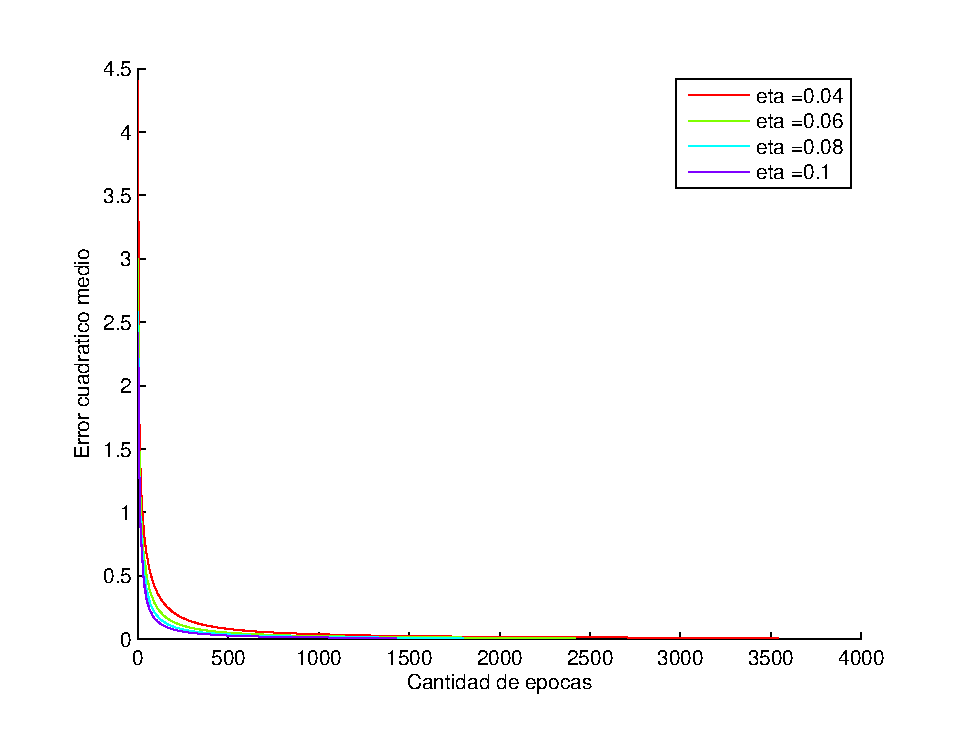
\includegraphics[scale=0.5]{images/PuriOr/OR_N5_err001_tanh.eps}
  \caption{Funci\'on OR, N = 5 y funci\'on de activaci\'on $g(h) = tanh(\beta h)$}
  \label{fig:tanh}
\end{figure}

\begin{figure}[!ht]
	\includegraphics[scale=0.5]{images/PuriOr/OR_N5_err001_lineal__error.eps}
  \caption{Funci\'on OR, N = 5 y funci\'on de activaci\'on $g(h) = h$}
  \label{fig:lineal}
\end{figure}

\begin{figure}[!ht]
	\includegraphics[scale=0.5]{images/PuriOr/OR_N5_err001_step.eps}
  \caption{Funci\'on OR, N = 5 y funci\'on de activaci\'on $g(h) = sgn(h)$}
  \label{fig:step}
\end{figure}

% --------------------- Con N = 3 --------------------------------
\begin{figure}[!ht]
	\includegraphics[scale=0.5]{images/PuriAnd/AND_N3_err001_tanh.eps}
  \caption{Funci\'on AND, N = 3 y funci\'on de activaci\'on $g(h) = tanh(\beta h)$}
  \label{fig:tanh}
\end{figure}

\begin{figure}[!ht]
	\includegraphics[scale=0.5]{images/PuriAnd/AND_N3_err001_lineal__error.eps}
  \caption{Funci\'on AND, N = 3 y funci\'on de activaci\'on $g(h) = h$}
  \label{fig:lineal}
\end{figure}

\begin{figure}[!ht]
	\includegraphics[scale=0.5]{images/PuriAnd/AND_N3_err001_step.eps}
  \caption{Funci\'on AND, N = 3 y funci\'on de activaci\'on $g(h) = sgn(h)$}
  \label{fig:step}
\end{figure}

\begin{figure}[!ht]
	\includegraphics[scale=0.5]{images/PuriOr/OR_N3_err001_tanh.eps}
  \caption{Funci\'on OR, N = 3 y funci\'on de activaci\'on $g(h) = tanh(\beta h)$}
  \label{fig:tanh}
\end{figure}

\begin{figure}[!ht]
	\includegraphics[scale=0.5]{images/PuriOr/OR_N3_err001_lineal__error.eps}
  \caption{Funci\'on OR, N = 3 y funci\'on de activaci\'on $g(h) = h$}
  \label{fig:lineal}
\end{figure}

\begin{figure}[!ht]
	\includegraphics[scale=0.5]{images/PuriOr/OR_N3_err001_step.eps}
  \caption{Funci\'on OR, N = 3 y funci\'on de activaci\'on $g(h) = sgn(h)$}
  \label{fig:step}
\end{figure}

\end{document}